\documentclass[tikz,border=2pt]{standalone}
\usepackage{pgfplots}
\pgfplotsset{compat=1.18}
\usetikzlibrary{positioning}
\usepackage{helvet}
\renewcommand{\familydefault}{\sfdefault}
\definecolor{ieeecolor}{HTML}{042C53}
\definecolor{jrnlcolor}{HTML}{378ADD}
\definecolor{othercolor}{HTML}{B4B2A9}
\definecolor{confcolor}{HTML}{D98B3F}
\begin{document}
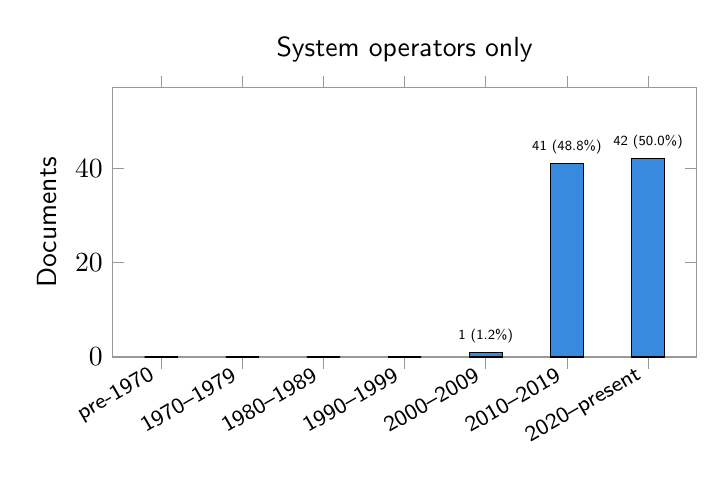
\begin{tikzpicture}
\begin{axis}[
    ybar, bar width=12pt,
    width=9cm, height=5cm,
    symbolic x coords={pre-1970,1970--1979,1980--1989,1990--1999,2000--2009,2010--2019,2020--present},
    xtick=data,
    x tick label style={rotate=30, anchor=east, font=\footnotesize},
    ylabel={Documents},
    ymin=0, ymax=57,
    axis line style={color=black!40},
    tick style={color=black!40},
    enlarge x limits=0.1,
    title={System operators only},
]
\addplot[fill=jrnlcolor] coordinates {(pre-1970,0) (1970--1979,0) (1980--1989,0) (1990--1999,0) (2000--2009,1) (2010--2019,41) (2020--present,42)};
\node[font=\tiny, anchor=south] at (axis cs:2000--2009,1) {1 (1.2\%)};
\node[font=\tiny, anchor=south] at (axis cs:2010--2019,41) {41 (48.8\%)};
\node[font=\tiny, anchor=south] at (axis cs:2020--present,42) {42 (50.0\%)};
\end{axis}
\end{tikzpicture}
\end{document}
